\documentclass[xcolor=dvipsnames, xetex,serif]{beamer}
%\documentclass[handout,xetex,serif]{beamer} %ใช้บรรทัดนี้สำหรับปริ้นเอกสาร
\usepackage{color,amsmath,graphics,graphicx}
\usepackage{epsfig,amsfonts,graphics}
\usepackage{mathrsfs,hyperref}
\usepackage{subcaption,float,framed,algorithm2e,hyperref}
%===============================================
\usepackage{fontspec,xltxtra,xunicode}
\defaultfontfeatures{Scale=1.23}
\XeTeXlinebreaklocale “th_TH” % สำหรับตัดคำ
\setmainfont[Scale=1.23]{THSarabunNew}
% 1.23 เท่าคือจาก 12 pt บน LaTeX ให้เท่ากับ 16pt บน Word
%=====================================================
%\usepackage{pgfpages} %ใช้บรรทัดนี้สำหรับปริ้นเอกสาร
%\pgfpagesuselayout{4 on 1}[a4paper,border shrink=5mm,landscape]
%\pgfpagesuselayout{2 on 1}[a4paper,border shrink=5mm]
 %ใช้บรรทัดนี้สำหรับปริ้นเอกสาร

%%%%%%%%%%%%%%% THEOREM Environments %%%%%%%%%% 					
\newtheorem{conjecture}[theorem]{บทคาดการณ์}								
\newtheorem{remark}[theorem]{หมายเหตุ}										
\numberwithin{equation}{section}							
\renewcommand\tablename{ตารางที่}
\renewcommand\figurename{รูปที่}						
\renewcommand{\bibname}{บรรณานุกรม}						
\renewcommand{\indexname}{ดรรชนี}
\setbeamertemplate{caption}[numbered]	
\setbeamertemplate{theorems}[numbered]				
%%%%%%%%%%%%%%%%%%%%%%%%%%%%%%%%%%%%%%%%%%%%%%%

\mode<presentation>{
	\usetheme{Madrid}
	\usecolortheme[named=PineGreen]{structure}}
 \title[วิธีเชิงตัวเลขสำหรับต่อเติมภาพ]{\normalsize{ขั้นตอนวิธีเชิงตัวเลขชนิดใหม่สำหรับการต่อเติมภาพที่ใช้การแปรผันรวมกับการประยุกต์สำหรับซ่อมแซมภาพจิตรกรรมไทยโบราณและการลบบทบรรยายจากอนิเมะ\\A new numerical algorithm for TV-based image inpainting with its applications for restoring ancient Thai painting images and removing subtitles from animes}}
 \author[ภัคพล]{ภัคพล พงษ์ทวี}
 \institute[SU]{
 	ภาควิชาคณิตศาสตร์\\
 	มหาวิทยาลัยศิลปากร \\}
 \date[Project Proposal]{การนำเสนอโครงร่างโครงงานวิจัย\\
 	5 ตุลาคม 2561}
 
 \AtBeginSubsection[]{
 	\begin{frame}<beamer>
 		\frametitle{Outlines}
 		\tableofcontents [currentsection,currentsubsection]
 	\end{frame}}
 	%\setbeamertemplate{item}[square]
 	%============================================================================
 	\begin{document}
 		\begin{frame}
 			\titlepage 
 			 \note{แนะนำตัว, วันนี้จะมานำเสนอหัวข้อวิจัยเรื่อง (ชื่อเรื่อง)}
 		\end{frame}
 		%\begin{frame} \tableofcontents \end{frame}
 		\section{Introduction}
		\begin{frame}
			\frametitle{ภาพดิจิตัล}
			\begin{figure}[H]
				\centering
				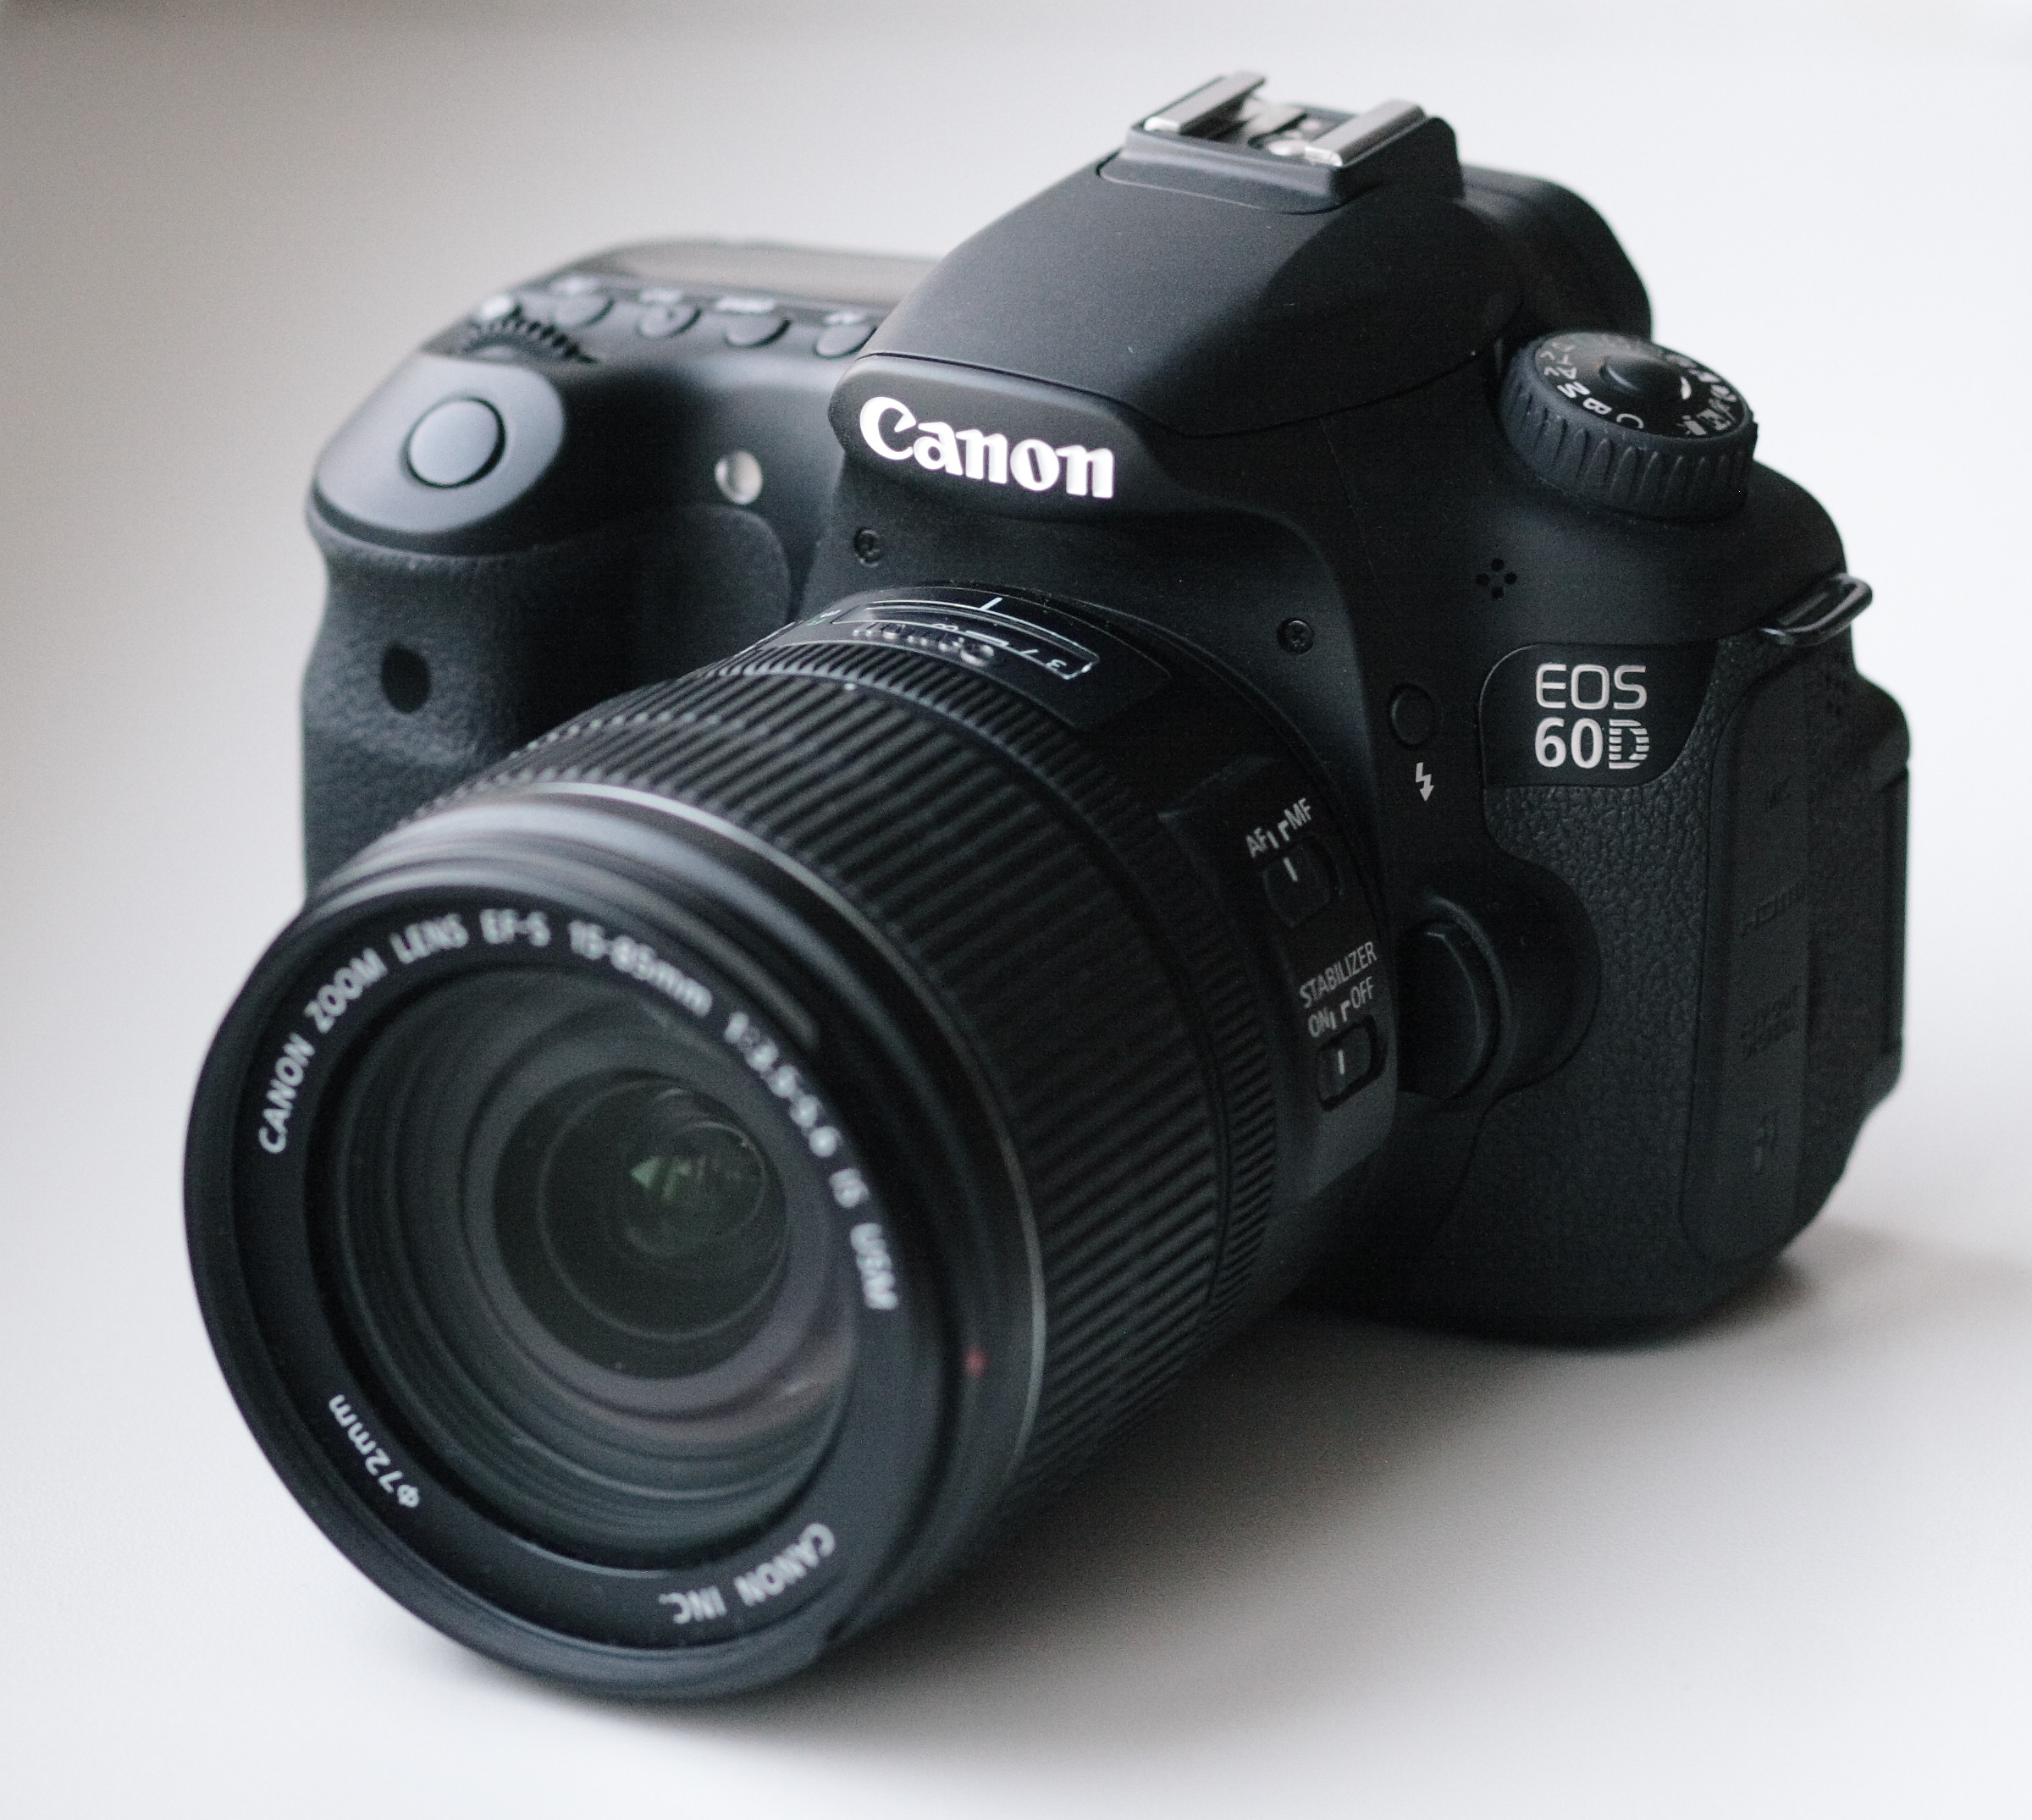
\includegraphics[width=0.4\linewidth]{images/camera-dslr.jpg}
				\caption{กล้องถ่ายภาพดิจิตัล สำหรับนำเข้าภาพดิจิตัล\footnote{ \tiny{ภาพจาก \url{https://commons.wikimedia.org/wiki/File:Canon_EOS_60D_01.jpg} สืบค้นเมื่อวันที่ 25 กันยายน 2561}}}
				\label{image:lightroom}
				%\note{ในปัจจุบันการใช้ภาพดิจิตัล ในสังคมเครือข่ายได้รับความนิยมอย่างแพร่หลาย สามารถรับส่งได้อย่างสะดวกและรวดเร็ว โดยนอกจากจะสามารถสร้างภาพดิจิตัลได้จากโทรศัพท์เคลื่อนที่แล้ว กล้อง DSLR กล้องดูดาว หรือแม้กระทั่งอุปกรณ์ทางการแพทย์}
			\end{figure}
		\end{frame} 		
		\begin{frame}
			\frametitle{การประมวลผลภาพ}
			\begin{figure}[H]
				\centering
				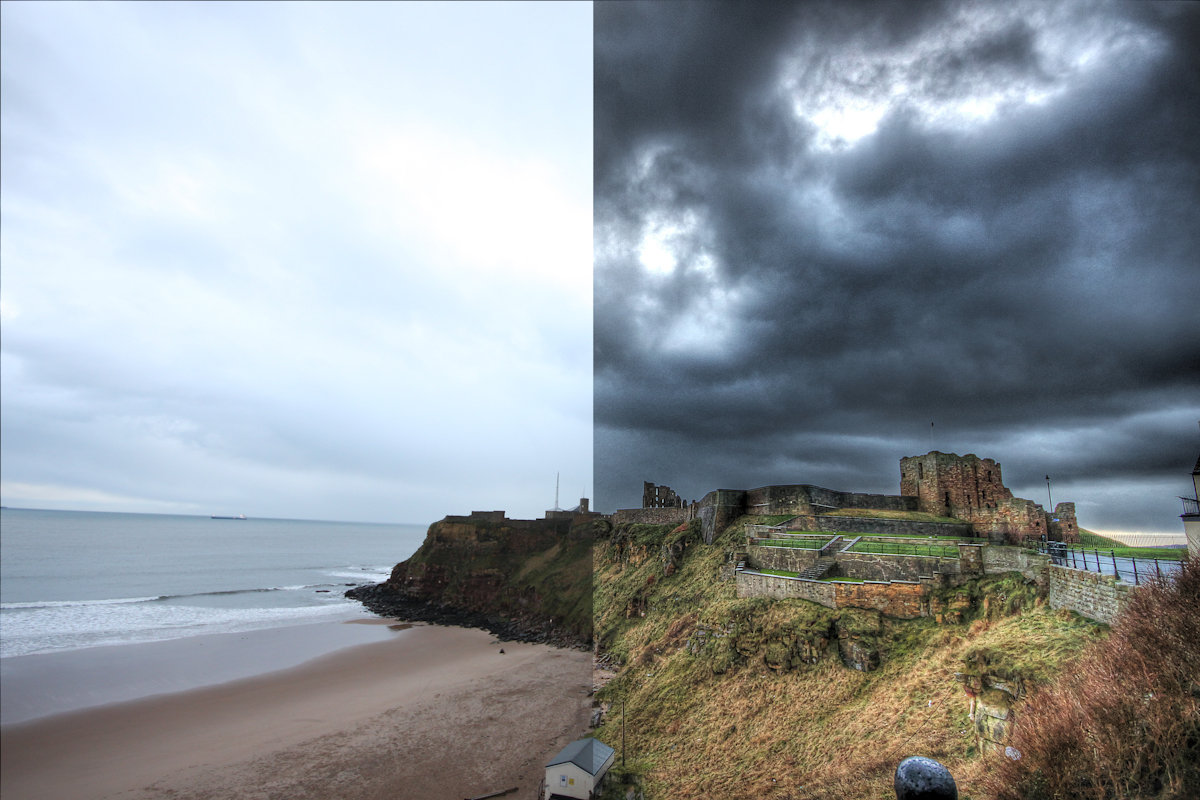
\includegraphics[width=0.6\linewidth]{images/lightroom.jpg}
				\caption{เปรียบเทียบภาพ ก่อน/หลัง การประมวลผล\footnote{ \tiny{ภาพจาก \url{https://commons.wikimedia.org/wiki/File:Before_and_after_HDR_(6747894381).jpg} สืบค้นเมื่อวันที่ 25 กันยายน 2561}}}
				\label{image:lightroom}
			\end{figure}
			%\note{ก่อนภาพจะถูกนำไปใช้ มักจะผ่านการประมวลผลภาพก่อนเสมอ ทั้งภาพตามสื่อสิ่งพิมพ์ต่างๆ ก่อนจะนำไปตีพิมพ์ก็จะนำมาประมวลผลเพื่อให้ได้ภาพที่สวยงาม คมชัดขึ้น หรือแม้กระทั่งภาพทางการแพทย์ก็จะมีการกำจัดสัญญาณรบกวนเพื่อให้สามารถหาสาเหตุของโรคได้ง่ายขึ้่น}
		\end{frame} 		
		\begin{frame}
		\frametitle{การต่อเติมภาพ (Image Inpainting)} 
			\begin{figure}[H]
				\centering
				\begin{subfigure}{0.3\linewidth}
					\centering
					
\includegraphics[width=0.8\linewidth]{images/grayscale_inpaint/toinpaint.png}
					\caption{ภาพที่ต้องการซ่อมแซม}
					%note{การต่อเติมภาพ เป็นวิธีการประมวลผลภาพชนิดหนึ่งมีเป้าหมายเพื่อซ่อมแซมภาพด้วยการต่อเติมข้อมูลของความเข้มของสีบนบริเวณที่กำหนด (ต่อไปจะเรียกบริเวณนี้ว่าโดเมนต่อเติม) โดยอาศัยข้อมูลของความเข้มของสีที่ปรากฏในภาพ จากภาพต้องการต่อเติมพื้นที่สีขาว ซึ่งเมื่อต่อเติมแล้วจะได้ภาพดังนี้}
				\end{subfigure}
				\begin{subfigure}{0.3\linewidth}
					\centering
					
\includegraphics[width=0.8\linewidth]{images/grayscale_inpaint/inpaintdomain.png}
					\caption{โดเมนต่อเติม}
				\end{subfigure}
				\begin{subfigure}{0.3\linewidth}
					\centering
					
\includegraphics[width=0.8\linewidth]{images/grayscale_inpaint/result_splitbergman.png}
					\caption{ภาพที่ได้รับการซ่อมแซม}
				\end{subfigure}
				\caption{ตัวอย่างการซ่อมแซมภาพ}
				\label{fig1}
			\end{figure}
		\end{frame} 		
		\begin{frame}
			\frametitle{การประยุกต์ใช้การต่อเติมภาพในปัจจุบัน}
			\begin{figure}[H]
				\centering
				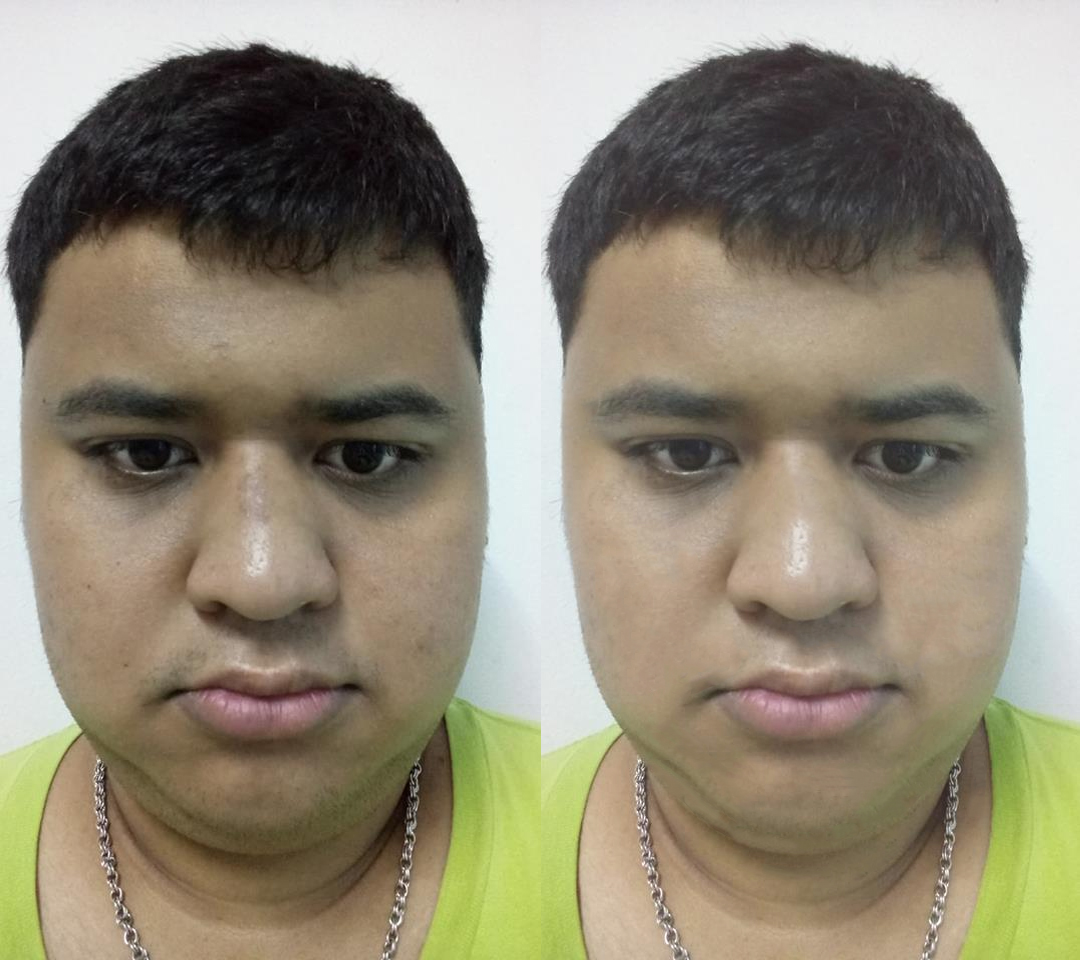
\includegraphics[width=0.6\linewidth]{images/self-beauty.jpg}
				\caption{เปรียบเทียบภาพ ก่อน/หลัง การใช้แอปพลิเคชัน snapseed}
				\label{image:self-beauty}
				% \note{ เท่าที่ผู้วิจัยศึกษาและค้นคว้ามาจนถึงขณะนี้ ผู้วิจัยพบว่าการต่อเติมภาพมักนิยมนำไปใช้งานสำหรับการปรับแต่งความสวยงามของภาพบุคคลที่ถ่ายจากโทรศัพท์เคลื่อนที่ เช่น การลบร่องรอยของรอยตีนกา การลบร่องรอยแผลเป็นที่เกิดจากสิวเสี้ยน (ให้ดูรอยสิวที่หายไป)}
			\end{figure}
		\end{frame} 		
		\begin{frame}
			\frametitle{การซ่อมแซมภาพจิตรกรรมไทยโบราณ}
			 \begin{figure}[h]
				\[
				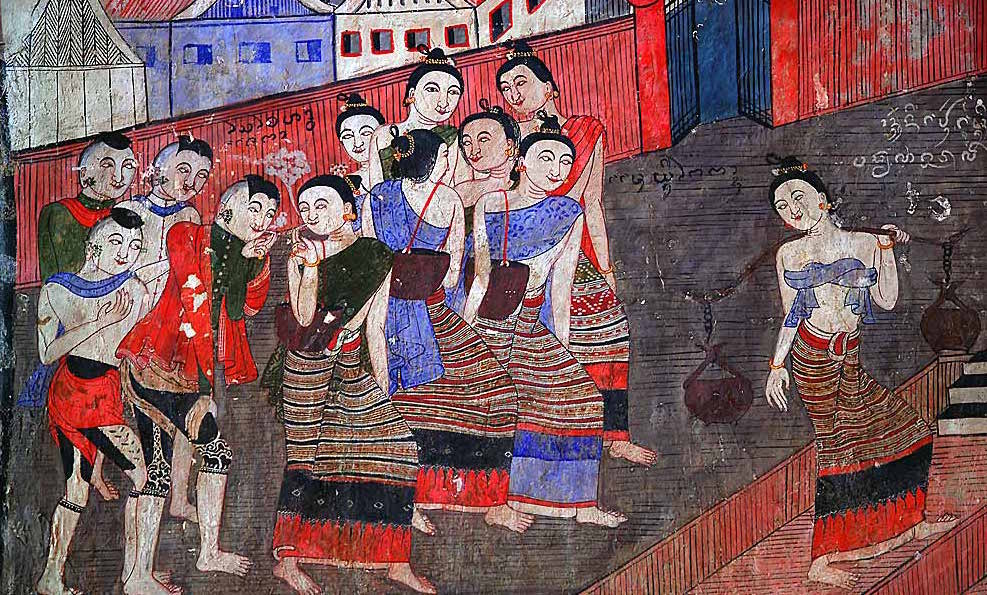
\includegraphics[width=0.6\linewidth]{images/thaiart.jpg}
				\]
				\caption{ภาพจิตรกรรมไทยที่วัดภูมินทร์ อำเภอเมือง จังหวัดน่าน\footnote{\tiny{ภาพถ่ายที่วัดภูมินทร์ อำเภอเมือง จังหวัดน่าน; ภาพจาก \url{http://topicstock.pantip.com/camera/topicstock/2009/02/O7514399/O7514399.html} สืบค้นเมื่อวันที่ 23 กันยายน 2561}}}
				\label{image:thaiart}
			\end{figure}
			%note{ภาพเขียนที่มีเอกลักษณ์ความเป็นศิลปะไทยซึ่งโดดเด่นและแตกต่างจากภาพเขียนของชนชาติอื่น อย่างไรก็ตาม ภาพจิตรกรรมไทยจำนวนไม่น้อยที่เสื่อมสลายตามกาลเวลา แต่การซ่อมแซมในบางครั้งอาจทำให้รายละเอียดในตัวภาพเขียนได้เปลี่ยนไป ก่อให้เกิดความเสียหายที่ประเมินค่าไม่ได้ เนื่องจากเป็นการซ่อมแซมโดยการใช้ขั้นตอนวิธีเชิงตัวเลขบนภาพดิจิตัลซึ่งเป็นสำเนาของภาพเดิม ด้วยเหตุผลดังกล่าว ผู้วิจัยได้เล็งเห็นว่าการซ่อมแซมภาพจิตรกรรมไทยโบราณมีความจำเป็นเร่งด่วน เนื่องจากภาพที่ได้รับการซ่อมแซมด้วยการต่อเติมภาพสามารถนำไปใช้ประกอบการตัดสินใจเพื่อวางแผนก่อนการลงมือซ่อมแซมภาพเขียนจริงได้  นอกจากนี้ ขั้นตอนวิธีการต่อเติมภาพสามารถนำไปใช้สร้างแอปพลิเคชันบนโทรศัพท์เคลื่อนที่เพื่อในไปใช้เป็นข้อมูลในการเข้าชมภาพเขียนเดิมที่ยังไม่ได้รับการซ่อมแซมและภาพเขียนที่ได้รับการซ่อมแซมโดยวิธีการทางคณิตศาสตร์จากแอปพลิเคชันที่พัฒนาขึ้น}
		\end{frame} 
		\begin{frame}
			\frametitle{ความท้าทายในการซ่อมแซมภาพจิตรกรรมไทยโบราณ}
			\begin{itemize}
				\item [(1)] ความสามารถของช่างฝีมือที่เปลี่ยนไปตามยุคสมัย
				\item [(2)] ไม่มีภาพต้นฉบับสำหรับเปรียบเทียบผลลัพธ์เพื่อใช้ซ่อมแซม	
				\item[(3)] สีที่ใช้งานในปัจจุบันไม่เหมือนกับในอดีต	
			\end{itemize}		
		\end{frame} 
		\begin{frame}
			\frametitle{การลบบทบรรยายบนอนิเมะ}
			 \begin{figure}[h]
				\[
				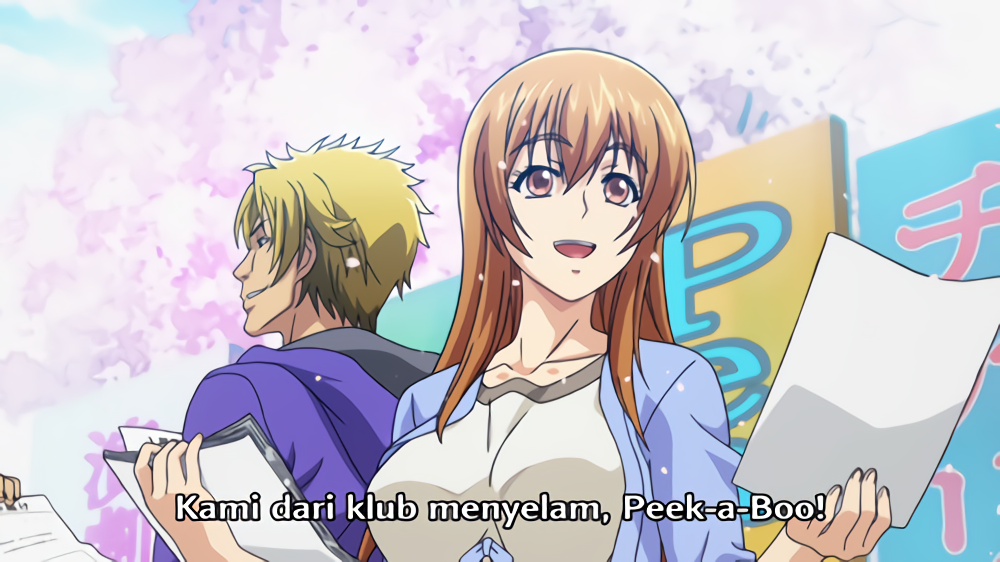
\includegraphics[width=0.6\linewidth]{images/anime-sub.png}
				\]
				\caption{เฟรมของอนิเมะที่มีบทบรรยายแบบแข็ง\footnote{\tiny{ภาพจาก \url{https://www.samehadaku.tv/2018/07/grand-blue-episode-1-subtitle-indonesia.html} สืบค้นเมื่อวันที่ 23 กันยายน 2561}}}
				\label{image:anime-sub}
				%\note{อนิเมะคือวิดีโอภาพวาดการ์ตูนสไตล์ญี่ปุ่นซึ่งเป็นที่นิยมของเยาวชนไทย ในการรับชมอนิเมะ แม้ว่าเยาวชนไทยสามารถรับชมด้วยบทพากย์เสียงภาษาไทย แต่ก็สูญเสียอรรถรสของการรับชมจากบทบรรยายแบบแข็งที่เป็นภาษาต่างประเทศในบริเวณด้านล่างของจอภาพ}
			\end{figure}
		\end{frame} 
		\begin{frame}
			\frametitle{ความท้าทายในการลบบทบรรยายออกจากอนิเมะ}
			\begin{itemize}
				\item [(1)] อนิเมะเป็นวิดีโอซึ่งแสดงผลประมาณ 24 เฟรม(ภาพ)ต่อวินาที
				\item [(2)] แต่ละเฟรมอาจมีหรืออาจไม่มีบทบรรยายก็ได้
				\item [(3)] แต่ละเฟรมอาจมีหรืออาจไม่มีบทบรรยายเดียวกันก็ได้
				\item [(4)] แต่ละเฟรมเป็นการแสดงผลภาพสีที่มีระดับความคมชัดสูง (high definition) ขนาดมากถึง $1920\times1080$ พิกเซล
			\end{itemize}
			%note{อนิเมะด้วยการลบบทบรรยายภาษาต่างประเทศจึงเป็นงานที่ยุ่งยากและท้าท้ายมาก เนื่องจาก (อ่านเลย lol)}
		\end{frame} 
		\begin{frame}
			\frametitle{การสร้างตัวแบบทางคณิตศาสตร์}
			\begin{itemize}
				\item การต่อเติมสำหรับภาพเฉดเทา
				\item การต่อเติมสำหรับภาพสี
			\end{itemize}
		\end{frame}
		\begin{frame}
			\frametitle{ภาพเฉดเทา}
			\begin{itemize}
				\item โดเมนภาพ (image domain) $\Omega \subset \mathbb{R}^2$ 
				\item โดเมนต่อเติม (inpainting domain)  $ D \subset \mathbb{R}^2$
				\item พิกัดทางกายภาพ (physical position) $ \mathbf{x} = (x,y) \in \Omega $ 
				\item ระดับความเข้มของภาพ (image intensity)  $V \subset [0,\infty)$ 
				\item ภาพเฉดเทา (grayscale image) $ u: \Omega \rightarrow V,\ z: \Omega \rightarrow V$
				\item โดยไม่เสียหลักการสำคัญ $ \Omega = [1,n]^2 $ และ $ V = [0,1] $ เมื่อ $n>0$ เป็นจำนวนเต็มบวก 
			\end{itemize}
			 \begin{figure}[h]
				\[
				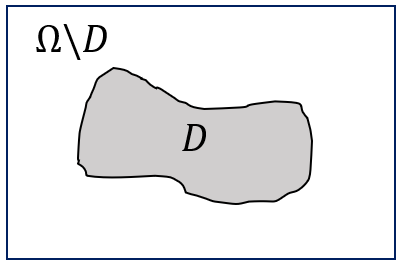
\includegraphics[width=0.3\linewidth]{images/sample-domain.png}
				\]
				\caption{$D$ แทนโดเมนต่อเติม}
				\label{image:sample-domain}
			\end{figure}
			%note{ในการกล่าวถึงขั้นตอนวิธีการต่อเติมภาพ จะเริ่มต้นด้วยการกล่าวทบทวนเกี่ยวกับการต่อเติมภาพเฉดสีเทา โดยขอกำหนดตัวแปรต่างๆ ดังนี้}
		\end{frame} 
		\begin{frame}
			\frametitle{ตัวแบบการต่อเติมภาพเฉดสีเทาที่ใช้การแปรผันรวม}
			\begin{align*}
			\min_{u} \{ \mathcal{J}(u) = \frac{1}{2} \int_{\Omega}\lambda (u-z)^2 d\Omega +  \int_{\Omega}  |\nabla u|  d\Omega \}
			\end{align*}
			 \vspace{1cm}
			\begin{align*}
			\lambda=\lambda(\mathbf{x}) = \left \{ \begin{array}{ll}  \lambda_0, & x \in \Omega \textbackslash D \\ 0, & x \in D  \end{array} \right . 
			\end{align*}
			\let\thefootnote\relax\footnotetext{\tiny{T.F. Chan and J. Shen , “Mathematical models of local non-texture inpaintings”, SIAM Journal on Applied Mathematics, vol. 62, no. 3, pp. 1019–1043, 2001.}}	
			%note{ในการต่อเติมภาพเฉดสีเทาคุณ Chan และ Shen  ได้นำเสนอตัวแบบเชิงการแปรผัน (variational model) ที่ใช้เร็กกิวลาร์ไรซ์เซชันแบบการแปรผันรวม โดยพัฒนาต่อจากตัวแบบ ROF ซึ่งใช้สำหรับการกำจัดสัญญาณรบกวน ซึ่งตัวแบบเชิงการแปรผันนี้กำหนดดังสมการนี้ และ lambda แทนพารามิเตอร์เร็กกิวลาร์ไรซ์เซชัน (regularization parameter) และ $\lambda_0 >0$}
		\end{frame} 
		\begin{frame}
			\frametitle{ตัวแบบการต่อเติมภาพเฉดสีเทาที่ใช้การแปรผันรวม (ต่อ)}
			\begin{align*}
			\min_{u} \{ \mathcal{J}(u) = \frac{1}{2} \int_{\Omega}\lambda (u-z)^2 d\Omega +  \int_{\Omega}  |\nabla u|  d\Omega \}
			\end{align*}
			$$ \Big \downarrow$$
			\begin{align*}
			\left \{ \begin{array}{ll}  - \nabla \cdot  \Big( \dfrac{\nabla u}{|\nabla u|} \Big) + \lambda (u-z) = 0,  & \hspace{1cm} \mathbf{x} \in (1,n)^2 \\ \dfrac{\partial u}{\partial \boldsymbol{n}} = 0, & \hspace{1cm} x \in \partial \Omega \end{array} \right .
			\end{align*}			
			%\note{โดยแคลคูลัสของการแปรผัน (Calculus of variations) จะได้สมการออยเลอร์ลากรางจ์ที่เกี่ยวข้องกัน ได้ดังนี้}
		\end{frame} 
		\begin{frame}
			\frametitle{การเดินเวลาแบบชัดแจ้ง (explicit time marching)}
			\begin{align*}
			u(\mathbf{x},t_{k+1})=u(\mathbf{x},t_{k})+\tau\left(\nabla \cdot\left(\dfrac{\nabla u (\mathbf{x},t_k)}{| \nabla u (\mathbf{x},t_k) | }\right) + \lambda(\mathbf{x})(u (\mathbf{x},t_k)-z(\mathbf{x})) \right)
			\end{align*}
			\begin{align*}
			u(\mathbf{x},t_0)=z \hspace{1cm} t_k=t_0+k\tau\ (\tau>0)  \hspace{1cm}  t_0=0
			\end{align*}
			\vspace{1cm}
			\begin{align*}
				u(\mathbf{x},t_0), u(\mathbf{x},t_1), u(\mathbf{x},t_2), u(\mathbf{x},t_3), ... ,  \textcolor{red}{u(\mathbf{x},t^{*})}
			\end{align*}
			\let\thefootnote\relax\footnotetext{\tiny{L. I. Rudin, S. Osher, E. Fatemi, “Nonlinear total variation based noise removal algorithms", Physica D: Nonlinear Phenomena, vol 60, issues 1–4, pp. 259-268, 1992.}}			
			%\note{ต่อไปจะกล่าวทบทวนวิธีการเชิงตัวเลขสำหรับแก้สมการเชิงอนุพันธ์ย่อย ซึ่งมีด้วยกันหลายวิธี  Rudin, Osher และ Fatemi ได้แนะนำวิธีการเชิงตัวเลขสำหรับการกำจัดสัญญาณรบกวนด้วยวิธีการเดินเวลาแบบชัดแจ้ง ซึ่งสามารถนำมาประยุกต์เพื่อใช้กับการต่อเติมภาพได้ เริ่มจากการแนะนําตัวแปรเวลาสังเคราะห์ จากนั้นหาคําตอบแบบสภาวะคงตัว เมื่อเวลาลู่เข้าสู่อนันต์}
		\end{frame} 
		\begin{frame}
			\frametitle{การทำซ้ำแบบจุดตรึง (fixed-point iteration)}
			\begin{align*}
				- \nabla\cdot\left(\dfrac{\nabla u^{[\nu+1]}}{{| \nabla u |}^{[v]} }\right) + \lambda(u^{[\nu+1]}-z)  = 0,\ u^{[0]}=z
			\end{align*}
			\vspace{1cm}
			\begin{align*}
			u^{[0]}, u^{[1]}, u^{[2]}, u^{[3]}, ..., \textcolor{red}{u^{*}}    
			\end{align*}
			\let\thefootnote\relax\footnotetext{\tiny{C.R. Vogel and M.E. Oman,“Iterative methods for total variation denoising", SIAM Journal on Scientific Computing. vol. 17, pp. 227-238, 1996.}}
			%\note{นอกจากนี้ยังมีคณะวิจัยของ Vogel และ Oman ได้แนะนำวิธีการทำซ้ำแบบจุดตรึงสำหรับการกำจัดสัญญาณรบกวนไว้ ซึ่งสามารถนำมาประยุกต์กับวิธีการต่อเติมภาพ เริ่มจากการแนะนำดัชนีการทำซ้ำแบบจุดตรึง u=0,1,2,... และนิยามรูปแบบการทำซ้ำโดย }
		\end{frame} 
		\begin{frame}
	\frametitle{ปัญหาเชิงตัวเลข}
	\begin{figure}[H]
		\centering
		
\includegraphics[width=0.2\linewidth]{images/grayscale_inpaint/result_splitbergman.png}
		\caption{ตัวอย่างภาพที่เกิดปัญหาเชิงตัวเลข}
		\label{image:rgb-space}
		\end{figure}
		\begin{align*}
			\tfrac{1}{| \nabla u |}=\tfrac{1}{\sqrt{u_x^2+u_y^2}} \rightarrow \infty
			\end{align*}
			\begin{align*}
			|\nabla u| \approx| \nabla u |_\beta=\sqrt{u_x^2+u_y^2+\beta},\ 0< \beta \ll 1
			\end{align*}
			% \note{แต่ในบริเวณที่ u มีความเข้มสีเป็นเอกพันธ์ุ จะทำให้ (ชี้บรรทัดบน) 1ส่วนขนาดของแกรด u ลู่ออกสู่อนันต์ เพื่อหลีกเลี่ยงปัญหาเชิงตัวเลขจะเกิดขึ้นใน เราจะใช้ (ชี้บรรทัดล่าง) การประมาณขนาดของแกรดโดยเพิ่ม beta เข้าไป โดยค่า beta นี้ มีค่าน้อยลงมากขึ้นเท่าไหร่ ความแม่นยำของตัวแบบยิ่งมีมากขึ้นเท่านั้น แต่ เรายังพบอีกว่าการแก้สมการยิ่งมีความยุ่งยากมากขึ้นสำหรับ beta น้อยๆ }
		\end{frame}
		\begin{frame}
			\frametitle{วิธีการสปริทเบรกแมน (Split Bregman method)}
			\begin{align*}
			\min_{u,\boldsymbol{w}} \{ \mathcal{J}(u,\boldsymbol{w}) = \dfrac{1}{2} \int_{\Omega} \lambda(u-z)^2 d\Omega +  \int_{\Omega}  |\nabla \boldsymbol{w}|  d\Omega + \frac{\theta}{2} \int_{\Omega} (\boldsymbol{w} - \nabla u + \boldsymbol{b}) d\Omega \}
			\end{align*}
			\let\thefootnote\relax\footnotetext{\tiny{T. Goldstein and S. Osher,“The Split Bregman Method for L1-Regularized Problems", SIAM Journal on Imaging Sciences. vol. 2, issue 2, pp. 323-343, 2009.}}
			%\note{เพื่อเอาชนะความยากเชิงตัวเลขนี้ คณะวิจัยโดยคุณ Goldstein และ Osher ได้แนะนำวิธีการสปริทเบรกแมนซึ่งสามารถกล่าวถึงพอสังเขป โดยการใช้พารามิเตอร์เสริม w ในตัวแบบเชิงการแปรผัน และเพิ่ม b ซึ่งเป็นตัวแปร bergman}
		\end{frame} 
		\begin{frame}
			\frametitle{วิธีการสปริทเบรกแมน (ต่อ)}
				\begin{align*}
			\min_{u,\boldsymbol{w}} \{ \mathcal{J}(u,\boldsymbol{w}) = \dfrac{1}{2} \int_{\Omega} \lambda(u-z)^2 d\Omega +  \int_{\Omega}  |\nabla \boldsymbol{w}|  d\Omega + \frac{\theta}{2} \int_{\Omega} (\boldsymbol{w} - \nabla u + \boldsymbol{b}) d\Omega \}
			\end{align*}
			$$ \Big \downarrow$$
			\begin{align*}
			u^{\text{New}}=\underset{u}{\arg\min} \{ \mathcal{J}_1(u) = \dfrac{1}{2} \int_{\Omega} \lambda(u-z)^2 d\Omega + \frac{\theta}{2} \int_{\Omega} (\boldsymbol{w}^{\text{old}} - \nabla u + \boldsymbol{b}^{\text{old}}) d\Omega \}
			\end{align*}
			\begin{align*}
			\boldsymbol{w}^{\text{New}}=\underset{\boldsymbol{w}}{\arg\min} \{ \mathcal{J}_2(\boldsymbol{w}) = \int_{\Omega}  |\nabla \boldsymbol{w}|  d\Omega  + \frac{\theta}{2} \int_{\Omega} (\boldsymbol{w} - \nabla u^{\text{New}} + \boldsymbol{b}^{\text{old}}) d\Omega \}
			\end{align*}
			\begin{align*}
			\boldsymbol{b}^{\text{New}}=\boldsymbol{b}^{\text{old}}+\nabla u^{\text{New}}-\boldsymbol{w}^{\text{New}}
			\end{align*}
			%\note{เราจะใช้วิธีการหาค่าต่ำที่สุดแบบสลับ โดยทำการตรึงค่า w จากนั้นเริ่มแก้ปัญหาย่อย แล้วนำ u ที่ได้มาตรึงค่า u เพื่อแก้ปัญหาย่อย w จากนั้นจึงทำการเปลี่ยนค่าตัวแปร b แล้วเริ่มทำซ้ำที่การหา u ใหม่อีกครั้ง จนกระทั่งค่านอร์มระหว่างรูป u ปัจจุบันและก่อนหน้าน้อยกว่าค่าที่กำหนด}
		\end{frame}  
		\begin{frame}
			\frametitle{ภาพสี}
			\begin{figure}[H]
				\centering
				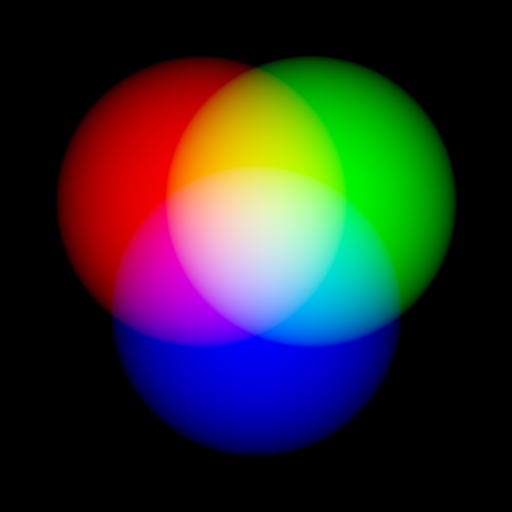
\includegraphics[width=0.4\linewidth]{images/rgb-space.png}
				\caption{ภาพสีเกิดจากการผสมกันระหว่างสี แดง เขียว และน้ำเงิน\footnote{\tiny{ภาพจาก \url{https://commons.wikimedia.org/wiki/File:Additive_RGB_Circles-48bpp.png}  สืบค้นเมื่อวันที่ 25 กันยายน 2561}}}
				\label{image:rgb-space}
			\end{figure}
		\end{frame}
		\begin{frame}
			\frametitle{ภาพสี (ต่อ)}
			\begin{align*}
				 \boldsymbol{u},\ \boldsymbol{z} : \Omega  \rightarrow V
			\end{align*}
			\begin{align*}
				\Big \downarrow
			\end{align*}
			\begin{align*}
				 \boldsymbol{u} = \begin{bmatrix} \textcolor{red}{u_1} \\ \textcolor{OliveGreen}{u_2} \\ \textcolor{blue}{u_3}   \end{bmatrix}, \ \boldsymbol{z} =\begin{bmatrix} \textcolor{red}{z_1} \\ \textcolor{OliveGreen}{z_2} \\ \textcolor{blue}{z_3} \end{bmatrix} : \Omega  \rightarrow V^3
			\end{align*} 
		\end{frame}
		\begin{frame}
			\frametitle{ตัวแบบการต่อเติมภาพสีที่ใช้การแปรผันรวม}
			\begin{align*}
			\min_{u} \{ \mathcal{J}(u) = \frac{1}{2} \int_{\Omega}\lambda (u-z)^2 d\Omega +  \int_{\Omega}  |\nabla u|  d\Omega \}
			\end{align*}
			\begin{align*}
			\Big \downarrow
			\end{align*}
			\begin{align*}
			\min_{u} \{ \mathcal{J}(u) = \underset{l=1}{\overset{3}{\sum}} 
			( \frac{1}{2} \int_{\Omega}\lambda (u_l-z_l)^2 d\Omega +  \int_{\Omega}  |\nabla u_l|  d\Omega ) \}
			\end{align*}
		\end{frame}
		\begin{frame}
		\frametitle{วิธีการสปริทเบรกแมนสำหรับภาพสี}
			\begin{align*}
			\min_{u,\boldsymbol{w}} \{ \mathcal{J}(u,\boldsymbol{w}) = \dfrac{1}{2} \int_{\Omega} \lambda(u-z)^2 d\Omega +  \int_{\Omega}  |\nabla \boldsymbol{w}|  d\Omega + \frac{\theta}{2} \int_{\Omega} (\boldsymbol{w} - \nabla u + \boldsymbol{b}) d\Omega \}
			\end{align*}
			\begin{align*}
			\Big \downarrow
			\end{align*}
			\begin{align*}
			\min_{\boldsymbol{u},\boldsymbol{w_1},\boldsymbol{w_2},\boldsymbol{w_3}} \{ \mathcal{J}(\boldsymbol{u},\boldsymbol{w_1},\boldsymbol{w_2},\boldsymbol{w_3}) &= \underset{l=1}{\overset{3}{\sum}} (  \dfrac{1}{2} \int_{\Omega} \lambda(u_l-z_l)^2 d\Omega +  \int_{\Omega}  |\nabla \boldsymbol{w_l}|  d\Omega \\ &+ \frac{\theta}{2} \int_{\Omega} (\boldsymbol{w_l} - \nabla u_l+ \boldsymbol{b_l}) d\Omega ) \}
			\end{align*}
		\end{frame}		
		\begin{frame}
			\frametitle{วัตถุประสงค์โครงการวิจัย}
			\begin{itemize}
				\item ศึกษาวิธีการแปรผันและขั้นตอนวิธีการเชิงตัวเลขสำหรับปัญหาการต่อเติมภาพเฉดสีเทา\\และภาพสีในระบบ RGB
				\item พัฒนาขั้นตอนวิธีการต่อเติมภาพชนิดใหม่สำหรับซ่อมแซมภาพจิตรกรรมไทย\\และลบบทบรรยายออกจากอนิเมะ
				\item นำขั้นตอนวิธีที่พัฒนาขึ้นไปใช้ในการซ่อมแซมภาพจิตรกรรมไทย\\และลบบทบรรยายในอนิเมะ
			\end{itemize}
		\end{frame}
		\begin{frame}
			\frametitle{ขอบเขตการศึกษา}
			\begin{itemize}
				\item ภาพจิตรกรรมไทยที่ใช้นำมาศึกษาและทดลองเป็นภาพจิตรกรรมไทยที่ได้มาอย่างถูกต้อง
				\item วิดีโอที่ใช้ศึกษาเป็นวิดีโอประเภทอนิเมะที่ได้มาอย่างถูกต้อง โดยศึกษากับไฟล์อนิเมะที่ใช้ปริภูมิสีแบบ RGB เท่านั้น
				\item บทบรรยายที่ใช้ทดสอบ จะถูกล้อมรอบไว้ด้วยสีดำ ขนาดความหนาขนาดไม่น้อยกว่า 5 พิกเซล
				\item วิดีโอที่ใช้ศึกษาขนาดไม่เกิน $1920\times1080$ พิกเซล
				\item คอมพิวเตอร์ที่ใช้ทดลองใช้หน่วยประมวลผล I7-6700HQ ใช้การ์ดจอ Nvidia GTX 960M แรม 16GB ฮาร์ดดิกส์แบบ SSD หรือดีกว่า
				\item คุณภาพของการซ่อมแซมภาพภาพและวิดีโอจะตรวจวัดโดยค่า PSNR SSIM RMSE 
				\item พารามิเตอร์เร็กกิวลาร์ไรซ์เซชัน $\lambda$ จะใช้แบบตรึงค่า การพัฒนาขั้นตอนวิธีเชิงอัตโนมัติเพื่อหาค่าที่เหมาะสมของ $\lambda$ ไม่อยู่ในขอบเขตการศึกษา
			\end{itemize}
		\end{frame}
		\begin{frame}
			\frametitle{วิธีการดำเนินงาน}
			\scalebox{0.7}{\begin{tabular}[ht]{|l|c|c|c|c|c|c|c|c|c|c|c|c|}
					\hline
					&\multicolumn{12}{c|}{เดือนที่}\\
					\cline{2-13}
					แผนการดำเนินงาน&1&2&3&4&5&6&7&8&9&10&11&12\\
					\hline
					ศึกษาตัวแบบและขั้นตอนวิธีการต่อเติมภาพที่ใช้การแปรผันรวมในเชิงลึก&x&x& & & & & & & & & &\\
					\hline
					พัฒนาขั้นตอนวิธีสำหรับการต่อเติมภาพที่ใช้การแปรผันรวมชนิดใหม่& & &x&x&x&x& & & & & &\\
					\hline
					ทดสอบขั้นตอนวิธีการต่อเติมภาพที่พัฒนาขึ้นโดยโปรแกรม- & & & &x &x&x& & & & & &\\
					คอมพิวเตอร์บนภาพสังเคราะห์และภาพจริง & & & & & & & & & & & &\\
					\hline
					อภิปรายผลที่ได้จากการทดลองเชิงตัวเลข & & & & & &x&x&x& & & &\\
					\hline
					สรุปผลการดำเนินงานวิจัยและจัดทำรูปเล่มฉบับสมบูรณ์& & & & & & & & &x&x&x&x\\
					\hline
			\end{tabular}}
		\end{frame}
		\begin{frame}
			\centering
			\Huge{ขอขอบคุณ}
		\end{frame}
	\end{document}





